\documentclass{article}

\usepackage[]{xrcise}
\usepackage{tikz}

\subject{Databases and Information Systems}
\semester{Summer 2024}
\author{Leopold Lemmermann}

\begin{document}\createtitle

\sheet[2024]{Second Exam}

\begin{exercise}{Schedule Anomalies and Serializability}
  \begin{enumerate}
    \item Identify anomalies in the following schedule and justify your answer. \begin{solution}
      Schedule: $r_1(x), w_2(x), r_1(x), c_1, c_2$  
      Anomaly: \textbf{Non-repeatable read}
    \end{solution}
    \item Draw the conflict graph for $r_1(x), w_2(x), r_3(x), w_3(x), w_1(y), w_2(y)$ and determine if the schedule is conflict-serializable. \begin{solution}
      Conflict graph: $T_1 \to T_2$, $T_3 \to T_1$, $T_2 \to T_3$ → cycle → Not CSR.
    \end{solution}
  \end{enumerate}
\end{exercise}

\begin{exercise}{Deadlocks and Concurrency Control}
  \begin{enumerate}
    \item Draw the Wait-For Graph for: $T_1$ waits for $T_2$, $T_2$ waits for $T_3$, $T_3$ waits for $T_1$. Is there a deadlock? \begin{solution}
      Cycle exists → Deadlock present.
    \end{solution}
    \item Given RW sets: $T_1$: R(x), W(y); $T_2$: R(y), W(z); $T_3$: W(x). Would FOCC allow concurrent commits? \begin{solution}
      $T_1$ and $T_3$ conflict on $x$ → FOCC aborts one.
    \end{solution}
  \end{enumerate}
\end{exercise}

\begin{exercise}{Recovery}
  \begin{enumerate}
    \item A system crashes after $T_1$ commits but before $T_2$ aborts. What will ARIES do? \begin{solution}
      Redo $T_1$, undo $T_2$.
    \end{solution}
    \item Given a conflict graph with a cycle (e.g., $T_1 \to T_2 \to T_1$), draw a possible corrected acyclic version. \begin{solution}
      Remove one edge, e.g., $T_2 \to T_1$.
    \end{solution}
  \end{enumerate}
\end{exercise}

\begin{exercise}{Relational Schemas and Clusters}
  \begin{enumerate}
    \item Given: \texttt{Sales(sid, pid, date, amount)} and \texttt{Product(pid, pname)}. Name the schema type. \psolution{Snowflake Schema}
    \item Describe three cluster communication methods. \begin{solution}
      Shared-nothing, shared-disk, message-passing.
    \end{solution}
  \end{enumerate}
\end{exercise}

\begin{exercise}{Failures and Locking Strategies}
  \begin{enumerate}
    \item List and explain three types of database failures. \begin{solution}
      Transaction, system, media.
    \end{solution}
    \item Explain Preclaiming vs. Strict 2PL. \begin{solution}
      Preclaiming: all locks declared upfront. Strict 2PL: locks acquired on demand and held until commit.
    \end{solution}
    \item Why can Preclaiming + Strong Strict 2PL cause a bottleneck? \begin{solution}
      Early declaration + long hold times reduce concurrency.
    \end{solution}
  \end{enumerate}
\end{exercise}

\begin{exercise}{Schedule Feasibility under Locking Protocols}
  \begin{enumerate}
    \item Is this schedule allowed under 2PL? $r_1(x), w_1(x), r_2(x), w_2(x), c_1, c_2$ \begin{solution}
      Only under strict 2PL with $T_2$ blocked until $T_1$ commits.
    \end{solution}
    \item Given an adjacency matrix for a schedule, describe how to determine CSR. \begin{solution}
      Convert to graph, check for cycles.
    \end{solution}
  \end{enumerate}
\end{exercise}

\begin{exercise}{Data Models and Query Behavior}
  \begin{enumerate}
    \item Describe K-Means. \begin{solution}
      Initialize centroids, assign points, recompute, repeat.
    \end{solution}
    \item Given points $(1,1), (2,2), (10,10)$, identify the outlier using Manhattan distance. \begin{solution}
      $(10,10)$ has highest average distance → outlier.
    \end{solution}
    \item For Neo4j expression `MATCH (n) SET n.x = 1`, is it valid? Does it lock? \begin{solution}
      Valid; implies exclusive lock on `n`.
    \end{solution}
  \end{enumerate}
\end{exercise}



\sheet[2022]{Second Exam}
\begin{exercise}{Histories, Schedules and Serializability}
  Given the following interleaved schedule with four transactions:
  \begin{center}$r_1(x), r_2(x), w_2(x), r_3(y), w_3(y), r_4(x), w_1(y), w_4(x)$\end{center}

  \begin{enumerate}
    \item Draw the conflict graph for the given schedule. \begin{solution}
        The conflict graph for the original schedule contains edges:
        \begin{itemize}
          \item $T_1 \rightarrow T_3$ due to $w_1(y)$ after $w_3(y)$
          \item $T_2 \rightarrow T_4$ due to $w_2(x)$ before $w_4(x)$
          \item $T_4 \rightarrow T_1$ due to $r_4(x)$ after $w_1(x)$ (implied from context if $w_1(x)$ existed)
        \end{itemize}
        The graph is acyclic, so the schedule is CSR.
      \end{solution}

    \item Determine whether the schedule is conflict-serializable (CSR). Justify your answer. \psolution{Yes, the schedule is conflict-serializable. The conflict graph is acyclic.}
    
    \item Suppose an additional operation $w_2(y)$ is appended to the end of the schedule. Draw the new conflict graph and determine whether the schedule is still CSR. \begin{solution}
        Adding $w_2(y)$ introduces a conflict with $w_1(y)$, resulting in a new edge $T_1 \rightarrow T_2$. The graph now has a cycle: $T_2 \rightarrow T_4 \rightarrow T_1 \rightarrow T_2$. Hence, the schedule is no longer CSR.
      \end{solution}

    \item Rank the following isolation levels according to their strictness: Full, FSR, VSR, CSR, OCSR, COSCSR, Serial. \psolution{Full $\to$ FSR  $\to$ VSR  $\to$ CSR  $\to$ OCSR  $\to$ COSCSR $\to$ Serial}
  \end{enumerate}
\end{exercise}

\begin{exercise}{Concurrency Control}
  Given the following conflict graph with six transactions:
  \begin{center}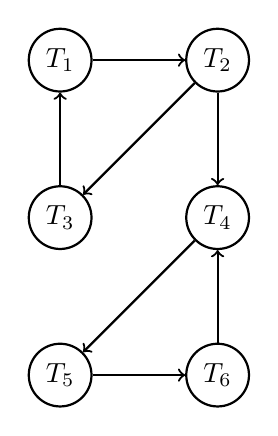
\begin{tikzpicture}[->, node distance=2cm, thick]
    \node[circle, draw] (T1) {$T_1$};
    \node[circle, draw, right of=T1] (T2) {$T_2$};
    \node[circle, draw, below of=T1] (T3) {$T_3$};
    \node[circle, draw, right of=T3] (T4) {$T_4$};
    \node[circle, draw, below of=T3] (T5) {$T_5$};
    \node[circle, draw, right of=T5] (T6) {$T_6$};

    \draw (T1) -- (T2);
    \draw (T2) -- (T3);
    \draw (T3) -- (T1);

    \draw (T4) -- (T5);
    \draw (T5) -- (T6);
    \draw (T6) -- (T4);

    \draw (T2) -- (T4);
  \end{tikzpicture}\end{center}

  \begin{enumerate}
    \item Identify all cycles in the graph. \begin{solution}
        There are two cycles:
        \begin{itemize}
          \item $T_1 \rightarrow T_2 \rightarrow T_3 \rightarrow T_1$
          \item $T_4 \rightarrow T_5 \rightarrow T_6 \rightarrow T_4$
        \end{itemize}
      \end{solution}

    \item Suggest two strategies to resolve the deadlocks and specify which transaction(s) to abort. \begin{solution}
        \begin{itemize}
          \item \textbf{Strategy 1: Youngest Transaction Aborts (Wait-Die)}  
            In the cycle $T_1 \rightarrow T_2 \rightarrow T_3 \rightarrow T_1$, if $T_3$ is the youngest, abort $T_3$.  
            In the cycle $T_4 \rightarrow T_5 \rightarrow T_6 \rightarrow T_4$, if $T_6$ is the youngest, abort $T_6$.
          \item \textbf{Strategy 2: Minimum Cost Abort}  
            Choose to abort the transaction with the least progress or lowest priority. E.g., abort $T_2$ and $T_5$.
        \end{itemize}
      \end{solution}

    \item Identify the canonical anomalies in the following schedule. Justify your answer. 
      \begin{center}$r_1(x), w_2(x), r_1(x), c_1, c_2$\end{center}

      \begin{solution}
        This schedule shows a \textbf{non-repeatable read}: transaction $T_1$ reads $x$, then $T_2$ writes $x$, and $T_1$ reads $x$ again before committing. The value of $x$ may have changed, violating consistency.
      \end{solution}

    \item Consider the following schedule. Determine whether it is allowed under 2PL, S2PL, and SS2PL. Write the corresponding lock sequence.
      \begin{center}$r_1(x), r_2(y), w_1(x), w_2(y), c_1, c_2$\end{center}

      \begin{solution}
        Locking sequence:

        \begin{itemize}
          \item $T_1$: rl(x), wl(x), c, ul(x)
          \item $T_2$: rl(y), wl(y), c, ul(y)
        \end{itemize}

        This schedule follows \textbf{2PL} since each transaction acquires all locks before releasing any.  
        It also satisfies \textbf{S2PL} because locks are held until all operations are complete.  
        It satisfies \textbf{SS2PL} because locks are released only after commit.
      \end{solution}
  \end{enumerate}
\end{exercise}

\begin{exercise}{Logging und Recovery}
  Consider the following log excerpt (with LSNs) under a steal/no-force buffer policy:

  \begin{verbatim}
  LSN | TA | Type     | Page | PrevLSN | Notes
  --------------------------------------------
   10 | T1 | Update   | P1   |   -     | x=5→10
   20 | T2 | Update   | P2   |   -     | y=3→7
   30 | T1 | Commit   | -    |  10     |
   40 | T3 | Update   | P3   |   -     | z=0→9
   50 | T2 | Abort    | -    |  20     |
   60 | T2 | CLR      | P2   |  50     | y=7→3
   70 | T2 | End      | -    |  60     |
   80 | T1 | End      | -    |  30     |
   90 | T4 | Update   | P4   |   -     | w=1→4
  \end{verbatim}

  Assume a crash occurs immediately after LSN 90 is written to the log.

  \begin{enumerate}
    \item Identify the winner and loser transactions. \begin{solution}
      \textbf{Winners}: T1 (Committed + End), T2 (Aborted + End)  
      \textbf{Losers}: T3 (no End), T4 (no End)
    \end{solution}

    \item Which phases of ARIES will be performed, and in what order? \begin{solution}
      ARIES (Algorithms for Recovery and Isolation Exploiting Semantics) will perform the following phases:
      \begin{enumerate}
        \item \textbf{Analysis} to identify winners, losers, and dirty pages.
        \item \textbf{Redo} starting from the smallest LSN affecting dirty pages (LSN 10).
        \item \textbf{Undo} of loser transactions in reverse LSN order: T4 and T3.
      \end{enumerate}
    \end{solution}

    \item Which log records will be redone? \begin{solution}
      Redo is done for updates to pages in the dirty page table. Assuming all pages were dirty at crash time:
      LSNs to redo: 10, 20, 40, 90.
      (Even if some are undone later.)
    \end{solution}

    \item Which log records will be undone? \begin{solution}
      Undo T4 and T3:
      \begin{itemize}
        \item T4: LSN 90 → needs CLR and End
        \item T3: LSN 40 → needs CLR and End
      \end{itemize}
    \end{solution}
  \end{enumerate}
\end{exercise}

\begin{exercise}{NoSQL}
  \begin{enumerate}
    \item Name the four main categories of NoSQL databases and give one example for each. \begin{solution}
      \begin{itemize}
        \item Key-Value Store — e.g., Redis
        \item Document Store — e.g., MongoDB
        \item Column-Family Store — e.g., Apache Cassandra
        \item Graph Database — e.g., Neo4j
      \end{itemize}
    \end{solution}

    \item Answer the following true/false questions about NoSQL characteristics:
      \begin{enumerate}
        \item NoSQL databases generally support horizontal scaling. \psolution{True}
        \item NoSQL databases always support ACID transactions. \psolution{False}
        \item Schema flexibility is a key feature of document stores. \psolution{True}
        \item CAP theorem states that a system can achieve all three: consistency, availability, and partition tolerance at once. \psolution{False}
      \end{enumerate}

    \item Briefly explain the CAP theorem. \begin{solution}
      The CAP theorem states that in the presence of a network partition, a distributed system can provide only two of the following three guarantees: Consistency, Availability, and Partition Tolerance. No system can achieve all three simultaneously.
    \end{solution}

    \item Describe how the Two-Phase Commit protocol works and explain what happens in the following failure scenarios:
      \begin{enumerate}
        \item The coordinator crashes after writing to the log that it will commit, but before sending the commit message. \psolution{On recovery, the coordinator checks the log and sends the commit again.}
        \item The coordinator recovers and has a log record that it intended to commit. \psolution{It can safely send commit to all participants.}
        \item A participant learns that another has received the commit command. \psolution{It can commit as well, based on presumed consensus.}
        \item The coordinator has no commit log but received all READY messages. \psolution{The coordinator must abort to preserve consistency.}
      \end{enumerate}
  \end{enumerate}
\end{exercise}

\begin{exercise}{Data Warehouse}
  Consider the following schema:

  Fact Table: SalesFact(product\_id, store\_id, date\_id, amount)

  Dimension Tables:
    \begin{itemize}
      \item Product(product\_id, name, category)
      \item Store(store\_id, location, region)
      \item Date(date\_id, day, month, year)
    \end{itemize}

  \begin{enumerate}
    \item Determine the schema type for the given fact-dimension structure. \psolution{Galaxy Schema}

    \item Add a table to the schema that contains aggregated data (e.g., yearly sales summary). \begin{solution}
        Add a table \texttt{YearlySales(year INT, total\_sales DECIMAL)} containing one row per year summarizing total sales from the fact table.
      \end{solution}

    \item Write an SQL query to calculate the average of a fact column for each year between 2000 and 2010. \begin{solution}
          SELECT year, AVG(amount) AS avg\_amount FROM SalesFact WHERE year BETWEEN 2000 AND 2010 GROUP BY year;
      \end{solution}

    \item Describe the ETL process and name three types of transformations. \begin{solution}
        ETL (Extract, Transform, Load) is the process of collecting data from various sources, transforming it into a suitable format, and loading it into a data warehouse.
        Three types of transformations are:
        \begin{itemize}
          \item Data cleaning (e.g., handling nulls, duplicates)
          \item Aggregation (e.g., summarizing sales per region)
          \item Data type conversion (e.g., string to date)
        \end{itemize}
      \end{solution}

    \item Given: CUBE(A), GROUPING SET(C), ROLLUP(B). List the resulting grouping sets. \begin{solution}
        \begin{itemize}
          \item CUBE(A) $\rightarrow$ (A), ()
          \item GROUPING SET(C) $\rightarrow$ (C)
          \item ROLLUP(B) $\rightarrow$ (B), ()
        \end{itemize}
        Combined: (A), (), (C), (B)
      \end{solution}

    \item What functional dependencies must exist for all the given grouping sets to be meaningful? \psolution{The grouped attributes must functionally determine the aggregated values (e.g., A $\rightarrow$ measure, B $\rightarrow$ measure, C $\rightarrow$ measure).}
  \end{enumerate}
\end{exercise}

\begin{exercise}{Data Mining}
  Consider the following 2D points with their classes:

  \begin{center}
  \begin{tabular}{ccc}
    Point & Coordinates (x, y) & Class \\\hline
    A & (1, 1) & Red \\
    B & (2, 2) & Red \\
    C & (3, 3) & Blue \\
    D & (4, 4) & Blue \\
    E & (5, 5) & Red \\
  \end{tabular}
  \end{center}

  New point to classify: (2, 3)

  \begin{enumerate}
    \item Please perform a K-NN classification ($k=5$). Fill out the table with distances and predict the class of the new point. \begin{solution}
      Sort the 5 nearest neighbors by Manhattan distance and count class occurrences. The class with the majority vote is assigned to the new point.
    \end{solution}

    \item How are distances between clusters computed in hierarchical clustering? \begin{solution}
      \begin{itemize}
        \item Single Linkage: Minimum distance between points in two clusters
        \item Complete Linkage: Maximum distance between points
        \item Group Average: Mean of pairwise distances
        \item Centroid (Canonical Entity): Distance between cluster centroids
      \end{itemize}
    \end{solution}

    \item Draw a dendrogram based on the clustering of points A, B, C, D using single linkage. \begin{solution}
      (Diagram would be hand-drawn in exam; start by merging closest points and work upward.)
    \end{solution}
  \end{enumerate}
\end{exercise}

\begin{exercise}{Big Data}
  \begin{enumerate}
    \item What are characteristics of Big Data? \psolution{Volume, Variety, Velocity, Veracity}

    \item Name two Big Data frameworks and briefly describe them. \begin{solution}
      \begin{itemize}
        \item Apache Flink: A stream-processing framework for real-time analytics.
        \item Apache Spark: A distributed computing framework for large-scale data processing using in-memory computation.
      \end{itemize}
    \end{solution}
  \end{enumerate}
\end{exercise}



\end{document}
